\clearpage
\sectionold{\RU{Простейшее четырехбайтное XOR-шифрование}\EN{Simplest possible 4-byte XOR encryption}}

\RU{Если при XOR-шифровании применялся шаблон длинее байта, например, 4-байтный, то его также легко
увидеть.}
\EN{If a longer pattern was used for XOR-encryption, for example a 4 byte pattern, it's easy
to spot as well.}
\RU{Например, вот начало файла kernel32.dll (32-битная версия из Windows Server 2008):}
\EN{For example, here is the beginning of the kernel32.dll file (32-bit version from Windows Server 2008):}

\begin{figure}[H]
\centering
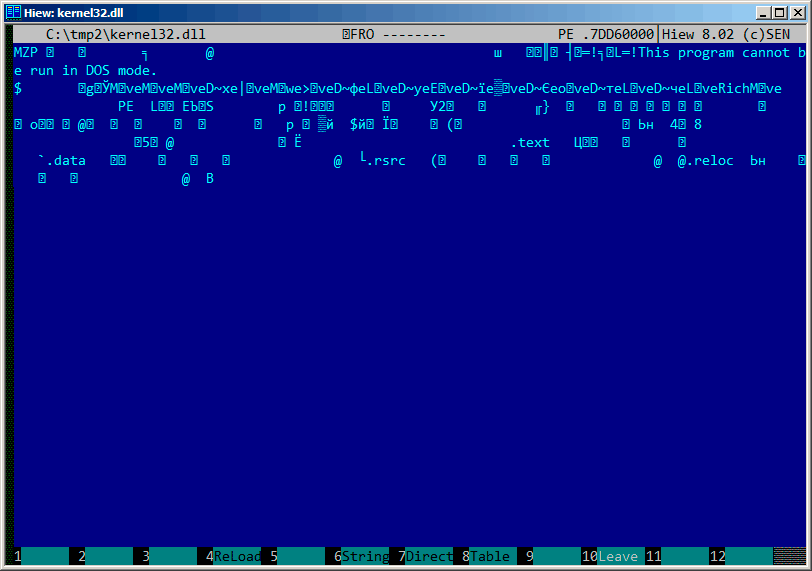
\includegraphics[scale=\FigScale]{ff/XOR/4byte/original1.png}
\caption{\EN{Original file}\RU{Оригинальный файл}}
\end{figure}

\clearpage
\RU{Вот он же, но \q{зашифрованный} 4-байтным ключем:}
\EN{Here it is \q{encrypted} with a 4-byte key:}

\begin{figure}[H]
\centering
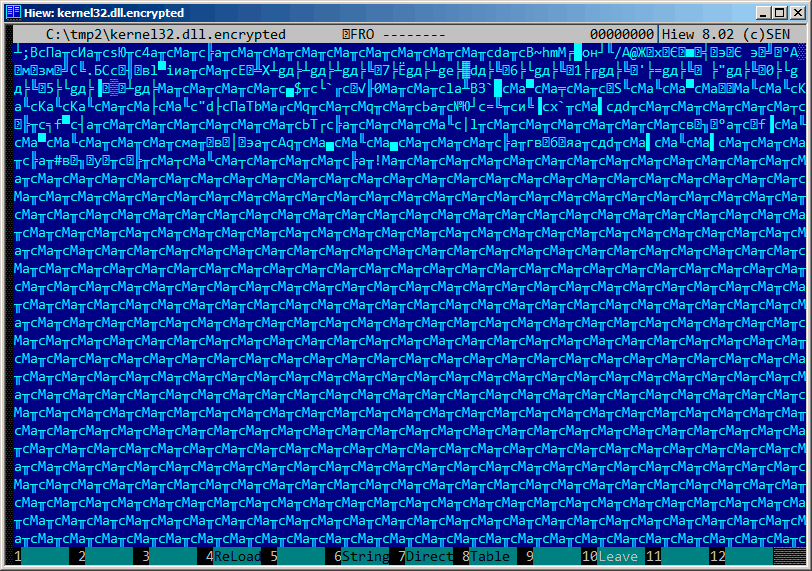
\includegraphics[scale=\FigScale]{ff/XOR/4byte/encrypted1.png}
\caption{\EN{\q{Encrypted} file}\RU{\q{Зашифрованный} файл}}
\end{figure}

\RU{Очень легко увидеть повторяющиеся 4 символа.}
\EN{It's very easy to spot the recurring 4 symbols.}
\RU{Ведь в заголовке PE-файла много длинных нулевых областей, из-за которых ключ становится видным.}
\EN{Indeed, the header of a PE-file has a lot of long zero areas, which are the reason for the key to become visible.}

\clearpage
\RU{Вот начало PE-заголовка в 16-ричном виде:}
\EN{Here is the beginning of a PE-header in hexadecimal form:}

\begin{figure}[H]
\centering
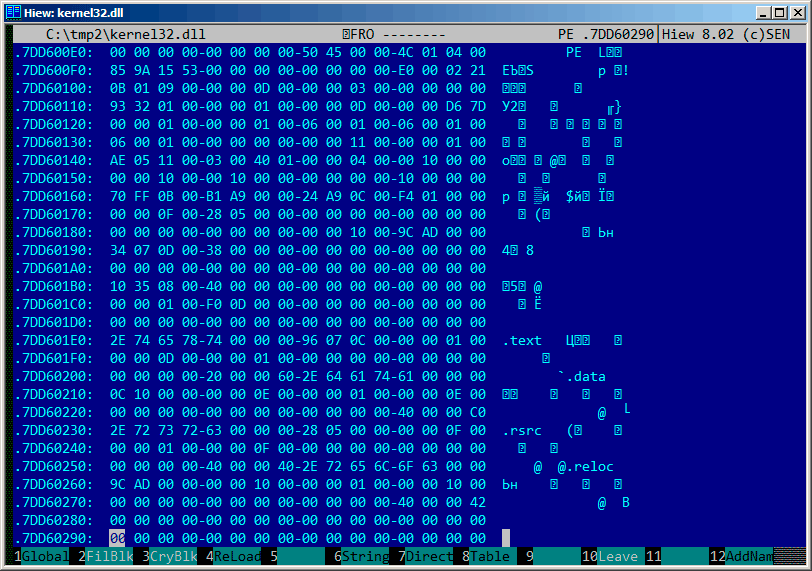
\includegraphics[scale=\FigScale]{ff/XOR/4byte/original2.png}
\caption{PE-\EN{header}\RU{заголовок}}
\end{figure}

\clearpage
\RU{И вот он же, \q{зашифрованный}:}
\EN{Here it is \q{encrypted}:}

\begin{figure}[H]
\centering
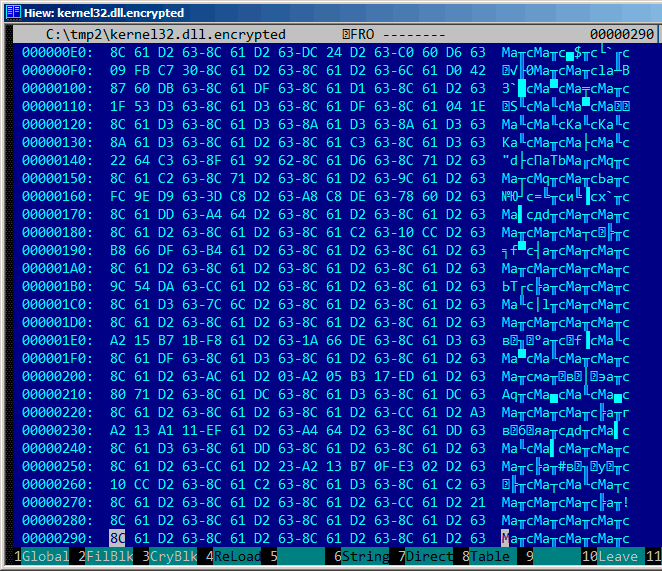
\includegraphics[scale=\FigScale]{ff/XOR/4byte/encrypted2.png}
\caption{\EN{\q{Encrypted} PE-header}\RU{\q{Зашифрованный} PE-заголовок}}
\end{figure}

\RU{Легко увидеть визуально, что ключ это следующие 4 байта}
\EN{It's easy to spot that the key is the following 4 bytes}: \TT{8C 61 D2 63}.
\RU{Используя эту информацию, довольно легко расшифровать весь файл.}
\EN{With this information, it's easy to decrypt the whole file.}

\RU{Таким образом, важно помнить эти свойства PE-файлов:
1) в PE-заголовке много нулевых областей;
2) все PE-секции дополняются нулями до границы страницы (4096 байт), 
так что после всех секций обычно имеются длинные нулевые области.}
\EN{So it is important to remember these properties of PE-files:
1) PE-header has many zero-filled areas;
2) all PE-sections are padded with zeroes at a page boundary (4096 bytes),
so long zero areas are usually present after each section.}

\RU{Некоторые другие форматы файлов могут также иметь длинные нулевые области.}
\EN{Some other file formats may contain long zero areas.}
\RU{Это очень типично для файлов, используемых научным и инженерным ПО.}
\EN{It's typical for files used by scientific and engineering software.}

\RU{Для тех, кто самостоятельно хочет изучить эти файлы, то их можно скачать здесь:}
\EN{For those who want to inspect these files on their own, they are downloadable here:}
\url{http://go.yurichev.com/17352}.

\subsectionold{\Exercise}

\begin{itemize}
	\item \url{http://challenges.re/50}
\end{itemize}

